\documentclass{szzclass}

\usepackage{amsmath}
\usepackage{graphics}
\usepackage[export]{adjustbox}[2011/08/13]

% \usepackage[czech]{babel}
% \usepackage[margin=3cm]{geometry}
% \usepackage{wrapfig}

% spacing
\usepackage{titlesec}
% \titlespacing*{\section}{0pt}{1ex}{0.5ex}
\titlespacing*{\subsection}{0pt}{1ex}{0ex}
\usepackage{dependencies/szz-math}

\topic{Limita a derivace funkce (definice a vlastnosti, geometrický význam),
využití při vyšetřování průběhu funkce.}
\author{Daniel Hampl}
\code{BI-SPOL-34}
\subject{ZMA}

\begin{document}
% \maketitle

\tableofcontents
\newpage

\section{Limita funkce}
\subsection{Definice}
Buďte $f$ reálná funkce reálné proměnné a 
$a \in \overline{\mathbb{R}}$. Nechť $f$ je definovaná na okolí bodu 
$a$, s možnou výjimkou bodu a samotného. Řekneme, že 
$c \in \overline{\mathbb{R}}$ je limitou funkce $f$ v bodě $a$, 
právě když pro každé okolí $H_c$ bodu $c$ existuje okolí 
$H_a$ bodu $a$ takové, že z podmínky $x \in H_a \backslash \{a\}$
plyne $f(x) \in H_c$. 

V symbolech:
\begin{center}
$(\forall H_c)(\exists H_a)(\forall x \in D_f)(x \in H_a \backslash \{a\} \implies f(x) \in H_c)$.
\end{center}


Tuto skutečnost zapisujeme:
\begin{center}
$\lim\limits_{x \rightarrow a} f(x) = c$, $\lim\limits_a f = c$.
\end{center}

\subsection{$\epsilon$-$\delta$ definice}

\begin{equation*}
\big(\forall\epsilon>0\big)\big(\exists\delta>0\big)\big( \forall x \in D_f)( 0 < |x - a| < \delta \ \Rightarrow \ |f(x) - c| < \epsilon\big).\end{equation*}

\subsection{Heineho věta}
$\lim\limits_{x \rightarrow a} f(x) = c$, právě když je $f$ definována
na okolí bodu $a$ (s možnou výjimkou bodu $a$) a pro každou posloupnost 
$(x_n)_{n=1}^\infty$ s limitou $a$ a splňující

\begin{center}
    $\{x_n \mid n\in\mathbb{N}\} \subset D_f \backslash \{a\}$
\end{center}
  
platí  
$\lim\limits_{x \rightarrow \infty} f(x_n) = c$.

\begin{figure}[h]
    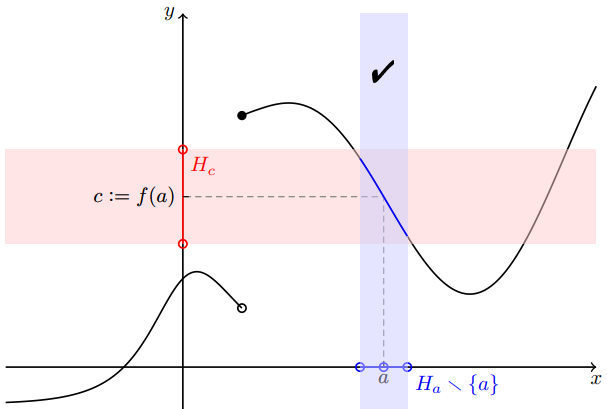
\includegraphics[width=.6\textwidth, center]{topics/bi-spol-34/images/nor_lim.png}
\end{figure}

\newpage

\subsection{Jednostraná limita}
Buďte $f$ reálná funkce reálné proměnné a $a \in \mathbb{R}$.
Nechť $f$ je definovaná na levém, resp. pravém, okolí bodu $a$.
Řekneme, že $c\in\overline{\mathbb{R}}$ je limitou funkce 
$f$ v bodě $a$ zleva, resp. zprava, právě když pro každé okolí 
$H_c$ bodu $c$ existuje levé okolí $H^−_a$, resp. pravé okolí 
$H^+_a$, bodu $a$ takové, že z podmínky 

\begin{center}
$x \in H^-_a \ \{a\}, \ \text{resp.} \ x \in H^+_a \ \{a\}$,
\end{center}
plyne
\begin{center}
$f(x) \in H_c$.
\end{center}
Zapisujeme
\begin{center}
$\lim\limits_{x\to a-} f(x) = c, \text{nebo} \lim\limits_{a-} f = c$,
\end{center}
resp.
\begin{center}
$\lim\limits_{x\to a+} f(x) = c, \text{nebo} \lim\limits_{a+} f = c$.
\end{center}

\subsection{Heineho věta pro jednostranné limity}
$\lim\limits_{x \rightarrow a_-} f(x) = c$, resp. 
$\lim\limits_{x \rightarrow a_+} f(x) = c$,
právě když je $f$ definována na levém, resp. 
pravém, okolí bodu $a$ a pro každou posloupnost 
$(x_n)_{n=1}^\infty$ s limitou $a$ a splňující

\begin{center}
    $\{x_n\, |\, n\in\mathbb{N}\} \subset D_f \cap (-\infty,a), \quad \textrm{resp.} \quad \{x_n\, |\, n\in\mathbb{N}\} \subset D_f \cap (a,+\infty)$,
\end{center}
  
platí  
$\lim\limits_{x \rightarrow \infty} f(x_n) = c$.

% \begin{figure}[h]
% 	\centering
% 	\begin{minipage}{0.3\textwidth}
%         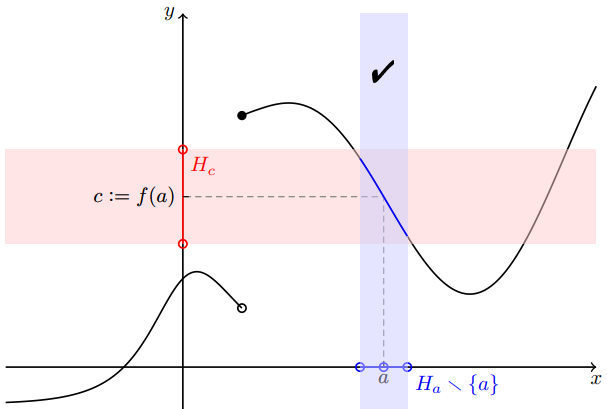
\includegraphics[width=\textwidth, center]{topics/bi-spol-34/images/nor_lim.png}
% 	\end{minipage}
% 	\begin{minipage}{0.3\textwidth}
%         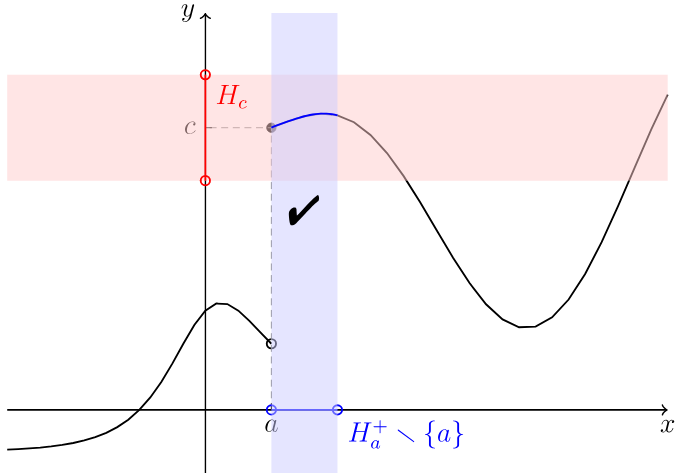
\includegraphics[width=\textwidth, center]{topics/bi-spol-34/images/jed_lim.png}
% 	\end{minipage}
% \end{figure}


\begin{figure}[h]
    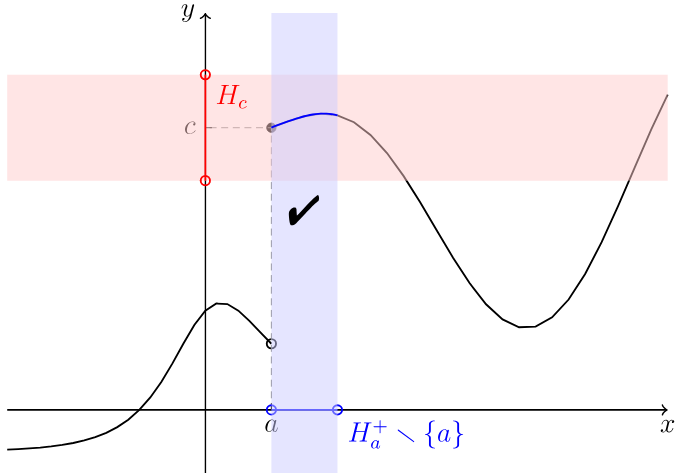
\includegraphics[width=.6\textwidth, center]{topics/bi-spol-34/images/jed_lim.png}
\end{figure}


\subsection{Vlastnosti}
Hodnota limity závisí na okolí bodu, nikoli na samotném bodě. Funkce $f$ v bodě $a$
ani nemusí být definovaná, přesto limita může existovat. Příkladem je funkce 
$f(x)\nolinebreak :=\nolinebreak \text{sgn} \frac{1}{x^2}$,
$D_f = \mathbb{R} \backslash \{0\}$.
Ačkoliv $0$ nepatří do $D_f$ platí $\lim\limits_{x\to 0} f(x) = 1$.

Nechť $a \in \mathbb{R}$. Limita $\lim\limits_{x \rightarrow a} f(x)$ existuje a je rovna c ∈ R, právě když existují obě
jednostranné limity $\lim\limits_{x \rightarrow a_+} f(x)$ a $\lim\limits_{x \rightarrow a_-} f(x)$ a obě jsou rovny c. 

\newpage

Nechť $f$ a $g$ jsou funkce, 
$a,b,c \in \overline{\mathbb{R}}$ a platí tři podmínky
\begin{itemize}
    \item $\displaystyle\lim_{x\to a} g(x) = b$,
    \item $\displaystyle\lim_{x\to b} f(x) = c$,
    \item buď $(\exists H_a)(\forall x\in D_g\cap H_a \backslash \{a\})(g(x) \neq b)$ nebo $(b\in D_f \ \text{a} \ f(b) = c)$.
\end{itemize}
Potom platí  $\displaystyle\lim_{x\to a} f(g(x)) = c$.


Nechť $f$ a $g$ jsou funkce a 
$a \in \overline{\mathbb{R}}$. Potom
\begin{equation*}
\begin{aligned} \lim_a (f + g) &= \lim_a f + \lim_a g, \\ \lim_a f \cdot g &= \lim_a f \cdot \lim_a g, \\ \lim_a \frac{f}{g} &= \frac{\lim_a f}{\lim_a g}, \end{aligned}\end{equation*}
platí v případě, že výrazy na pravé straně jsou definovány a v posledním případě za předpokladu, že 
$\frac{f}{g}$
je definována na okolí bodu 
$a$
s možnou výjimkou bodu 
$a$
samotného.

\subsection{Důsledek heineho věty}
Nechť 
$f$
 je funkce definovaná na okolí bodu 
a
$a\in\overline{\mathbb{R}}$
 a 
$(x_n)_{n=1}^\infty$
, 
$(z_n)_{n=1}^\infty$
 jsou dvě reálné posloupnosti patřící do 
$D_f$
, konvergující k 
$a$
 a splňující podmínky 
$x_n\neq a$
 a 
 $z_n\neq a$
 pro všechna 
$n\in\mathbb{N}$
. Pokud limity
$\lim\limits_{n\to\infty} f(x_n) \textrm{ a } \lim\limits_{n\to\infty} f(z_n)$
existují a jsou různé, nebo alespoň jedna z nich neexistuje, potom limita  
$\lim\limits_{x \rightarrow a} f(x)$
neexistuje.

\subsection{Nerovnost}

Mějme funkce $f$ a 
$g$ a nechť existují limity  
$\displaystyle\lim_{x\to a} f(x)$ a  
$\displaystyle\lim_{x\to a} g(x)$.
Pak platí následující dvě tvrzení:
\begin{itemize}
    \item Pokud $\displaystyle\lim_{x\to a} f(x) < \lim_{x\to a} g(x)$,
    potom existuje okolí $H_a$ bodu $a$ takové, že pro všechna
    $x\in H_a \backslash\{a\}$ platí $f(x) < g(x)$.
    \item Pokud existuje okolí $H_a$ bodu $a$ takové, že pro všechna
    $x\in H_a \backslash\{a\}$ je $f(x) \leq g(x)$, potom
    $\displaystyle \lim_{x\to a} f(x) \leq \lim_{x\to a} g(x)$.
\end{itemize}

\subsection{Limita sevřené funkce}

Nechť pro funkce $f$, $g$, $h$ a body $a, c \in \overline{\mathbb{R}}$ platí:
\begin{itemize}
    \item existuje okolí $H_a$ bodu $a$ takové, že pro každé $x\in H_a\backslash\{a\}$ platí $f(x) \leq g(x) \leq h(x)$
    \item existují $\displaystyle\lim_{x\to a}f(x) = \lim_{x\to a}h(x) = c$
\end{itemize}

Potom existuje i
$\displaystyle\lim_{x\to a} g(x)$
a je rovna $c$.

\newpage

\section{Derivace funkce}

\subsection{Definice}

Nechť $f$ je funkce definovaná na okolí bodu $a\in\mathbb{R}$. Pokud existuje limita


\begin{equation*}
\lim_{x\to a} \frac{f(x) - f(a)}{x-a}\end{equation*}
 
nazveme její hodnotu \textbf{derivací funkce} $f$ v bodě $a$
a označíme $f'(a)$. Pokud je tato limita konečná
(tj. $f'(a) \in \mathbb{R}$) řekneme, že funkce $f$
je diferencovatelná v bodě $a$.

Buď $f$ funkce s definičním oborem $D_f$. Nechť $M$
označuje množinu všech $a\in D_f$ takových, že existuje
konečná derivace $f'(a)$. Derivací funkce $f$ nazýváme
funkci s definičním oborem $M$, která každému $x \in M$
přiřadí $f'(x)$. Tuto funkci značíme symbolem $f'$.

\textbf{Další možná značení:}
\begin{equation*}
f'(a), \quad \dot{f}(a), \quad \frac{\mathrm{d}f}{\mathrm{d}x}(a).\end{equation*}

\begin{figure}[h]
    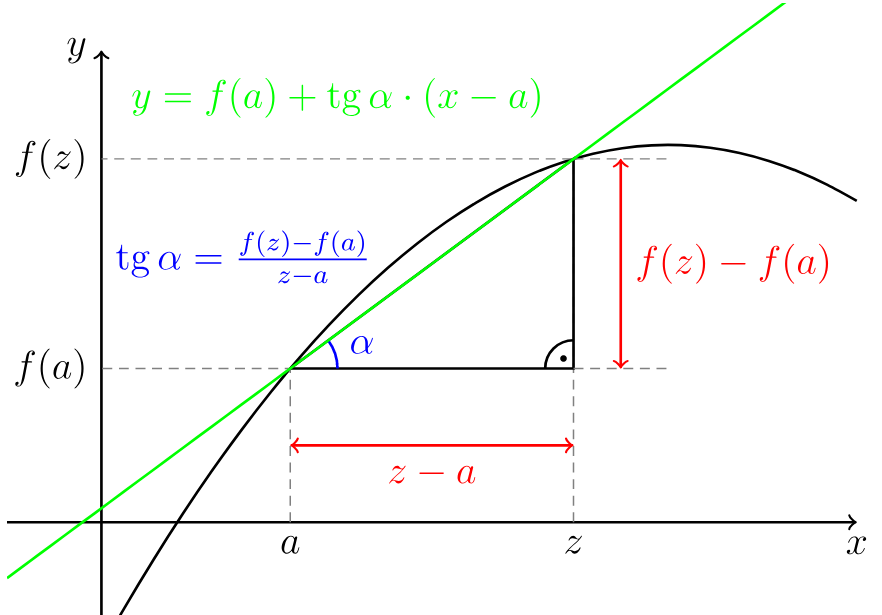
\includegraphics[width=.6\textwidth, center]{topics/bi-spol-34/images/tecna.png}
\end{figure}

\subsection{Tečna}
Nechť existuje $f'(a)$. Tečnou funkce $f$ v bodě $a$ nazýváme
\begin{itemize}
    \item přímku s rovnicí $x=a$ je-li funkce $f$ spojitá v bodě $a$ a $f'(a) = +\infty$ nebo $f'(a) = -\infty$.
    \item přímku s rovnicí $y = f(a) +  f'(a) (x-a)$ je-li $f'(a) \in\mathbb{R}$ (tj. je-li $f$ diferencovatelná v bodě $a$).
\end{itemize}

\newpage

\subsection{Operace}
\subsubsection{Sčítání, násobení, dělení}
Nechť funkce $f$ a $g$ jsou diferencovatelné v bodě $a$. Potom platí:
\begin{itemize}
    \item $(f+g)'(a) = f'(a) + g'(a)$
    \item $(f\cdot g)'(a) = f'(a) g(a) + f(a) g'(a)$
    \item $\displaystyle\left(\frac{f}{g}\right)'(a) = \frac{f'(a)g(a) - f(a)g'(a)}{g(a)^2}$, pokud $g(a) \neq 0$
\end{itemize}

\subsubsection{Složená funkce}
Nechť $g$ je funkce diferencovatelná v bodě $a$,
$f$ je diferencovatelná v bodě $g(a)$.
Potom funkce $f \circ g$ je diferencovatelná v bodě $a$
a platí
\begin{equation*}
(f \circ g)'(a) = f'\big( g(a) \big) \cdot g'(a).\end{equation*}

\subsubsection{Inverzní funkce}
Buďte $f$ spojitá a ryze monotónní na intervalu
$I=(a,b)$ a bod $c \in I$. Má-li inverzní funkce
$f^{−1}$ konečnou nenulovou derivaci v bodě $f(c)$,
potom má $f$ derivaci v bodě $c$ a platí
\begin{equation*}
f'(c) = \frac{1}{(f^{-1})'(f(c))}.\end{equation*}

\newpage

\section{Průběh funkce}

\subsection{Spojitost}

Nechť $f$ je reálná funkce reálné proměnné a nechť bod
$a \in D_f$. Řekneme, že funkce $f$ \textbf{je spojitá v bodě}
$a$ jestliže nastává alespoň jedna z následujících možností:

\begin{itemize}
    \item $\displaystyle \lim_{x\to a} f(x) = f(a)$,
    \item funkce $f$ je definována jen na pravém okolí bodu $a$, přesněji $(\exists H_a)(H_a \cap D_f = H^+_a)$, a $\displaystyle \lim_{x\to a+} f(x) = f(a)$,
    \item funkce $f$ je definována jen na levém okolí bodu $a$, přesněji $(\exists H_a)(H_a \cap D_f = H^-_a)$, a $\displaystyle \lim_{x\to a-} f(x) = f(a)$.
\end{itemize}

Funkce $f$ \textbf{je spojitá} v bodě $a$ \textbf{zprava}, pokud $\displaystyle\lim_{x\to a+} f(x) = f(a)$.\newline
Funkce $f$ \textbf{je spojitá} v bodě $a$ \textbf{zleva}, pokud $\displaystyle\lim_{x\to a-} f(x) = f(a)$.

Funkde $f$ \textbf{je spojitá na intervalu $J$}, právě kdyz je spojitá v každém bodě intervalu \textbf{$J$}.

\subsection{Extrémy funkce}

Řekneme, že funkce $f$ má v bodě $a \in D_f$
\begin{enumerate}
    \item lokální maximum
    \item lokální minimum
    \item ostré lokální maximum
    \item ostré lokální minimum
\end{enumerate}
právě když existuje okolí (v krajním bodě jednostranné) $H_a \subset D_f$ bodu $a$ tak, že
\begin{enumerate}
    \item pro všechna $x \in H_a$ platí $f(x) \leq f(a)$,
    \item pro všechna $x \in H_a$ platí $f(x) \geq f(a)$, 
    \item pro všechna $x \in H_a \backslash \{a\}$ platí $f(x) < f(a)$,
    \item pro všechna $x \in H_a \backslash \{a\}$ platí $f(x) > f(a)$,
\end{enumerate}

Nechť funkce $f$ má v bodě $a$ lokální extrém. Potom $f'(a)=0$,
nebo derivace v bodě $a$ neexistuje.

Funkce $f$ spojitá a definovaná právě na uzavřeném intervalu
$\langle a,b \rangle$ nabývá maxima a minima (tzv. globální extrém).
Extrém může být pouze v krajních bodech $a,b$ a
v bodech kde je derivace rovna $0$ nebo neexistuje.

\newpage

\subsection{Věty o přírustku funkce}
\subsubsection{Rolleova}
Nechť funkce $f$ splňuje podmínky
\begin{enumerate}
    \item $f$ je spojitá na intervalu $\langle a,b \rangle$,
    \item $f$ má derivaci v každém bodě intervalu $(a,b)$,
    \item $f$ $(a)=f(b)$.
\end{enumerate}
Potom existuje $c\in(a,b)$ tak, že $f'(c)=0$.


\begin{figure}[h]
    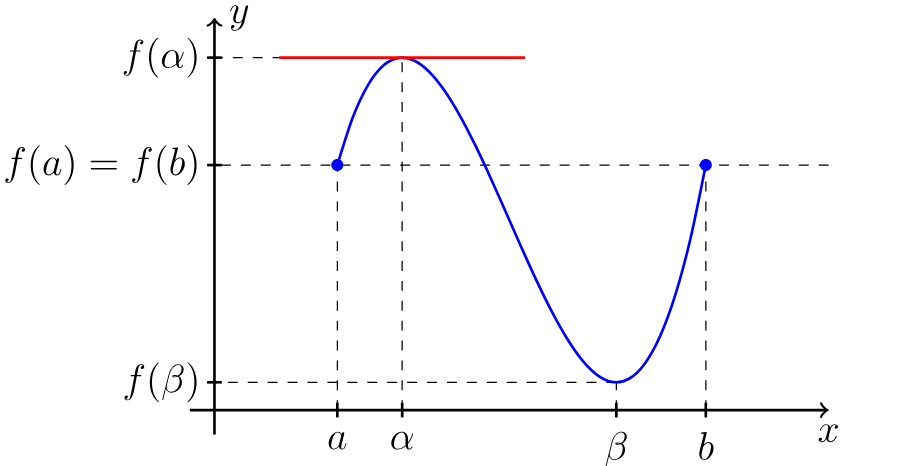
\includegraphics[width=.6\textwidth, center]{topics/bi-spol-34/images/roll.png}
\end{figure}


\subsubsection{Lagrangeova}
Nechť funkce $f$ splňuje podmínky
\begin{enumerate}
    \item $f$ je spojitá na intervalu $\langle a,b \rangle$,
    \item $f$ má derivaci v každém bodě intervalu $(a,b)$,
\end{enumerate}
Potom existuje bod $c \in (a,b)$ tak, že
$\displaystyle f'(c) = \frac{f(b) - f(a)}{b-a}$,
nebo ekvivalentně $f(b) - f(a) = f'(c) (b-a)$.
\begin{figure}[h]
    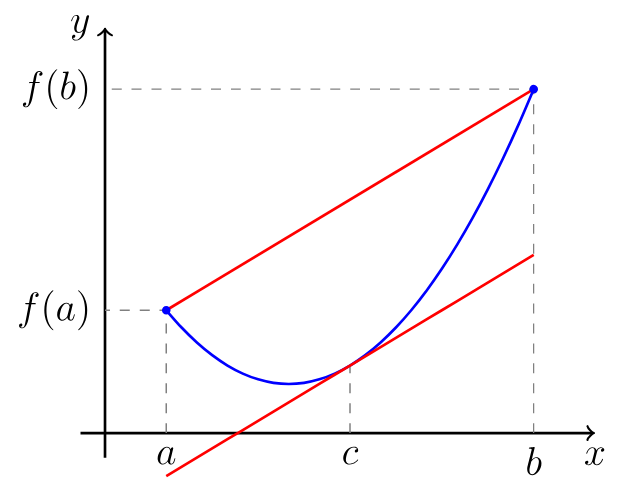
\includegraphics[width=.4\textwidth, center]{topics/bi-spol-34/images/lagrange.png}
\end{figure}

\subsection{Důsledky}
Nechť $J$ je interval s krajními body $a$ a $b$.
Potom vnitřkem intervalu $J$ nazveme otevřený
interval $(a,b)$. Značíme ho $J^\circ=(a,b)$.


\subsubsection{Rostoucí, klesající, konstantní}
Nechť $f$ je spojitá na intervalu $J$ a nechť pro
každé $x\in J^\circ$ existuje $f'(x)$. Potom platí
následujících pět tvrzení:
\begin{enumerate}
    \item $\big(\forall x\in J^\circ\big)\big(f'(x) \geq 0\big) \implies f$ je rostoucí  na $J$,
    \item $\big(\forall x\in J^\circ\big)\big(f'(x) \leq 0\big) \implies f$ je klesající na $J$,
    \item $\big(\forall x\in J^\circ\big)\big(f'(x) > 0\big) \implies f$ je ostře rostoucí  na $J$,
    \item $\big(\forall x\in J^\circ\big)\big(f'(x) < 0\big) \implies f$ je ste klesající na $J$,
    \item $\big(\forall x\in J^\circ\big)\big(f'(x) = 0\big) \implies f$ je konstantní na $J$.
\end{enumerate}



\subsubsection{Konvexní, konkávní}
Funkci $f$ definovanou na intervalu $J$ nazveme \textbf{konvexní na intervalu}
(resp. \textbf{konkávní na intervalu}) $J$, právě když pro každé $x_1,x_2,x_3 \in J$
splňující $x_1<x_2<x_3$, leží bod $(x_2,f(x_2))$ buďto pod (resp. nad) přímkou
spojující body $(x_1,f(x_1))$ a $(x_3,f(x_3))$, nebo na ní.

Funkci $f$ definovanou na intervalu $J$ nazveme \textbf{ryze konvexní na intervalu}
(resp. \textbf{ryze konkávní na intervalu}) $J$, právě když pro každé $x_1,x_2,x_3 \in J$
splňující $x_1<x_2<x_3$, leží bod $(x_2,f(x_2))$ buďto pod (resp. nad) přímkou
spojující body $(x_1,f(x_1))$ a $(x_3,f(x_3))$.

Buď $f$ funkce spojitá na intervalu $J$, která má druhou derivaci v každém bodě intervalu $J^\circ$.
\begin{itemize}
    \item Funkce $f$ je konvexní na intervalu $J$, právě když $f''(x)\geq0$pro každé $x\in J^\circ$.
    \item Je-li $f''(x)>0$ v každém bodě $x\in J^\circ$, pak je $f$ ryze konvexní na $J$.
\end{itemize}


Nechť funkce $f$ má konečnou derivaci v bodě $a\in D_f$.
Pokud existuje okolí $H_a$ bodu a takové, že pro všechna
$x\in H_a \backslash {a}$ leží všechny body $(x,f(x))$
nad (resp. pod) tečnou funkce $f$ v bodě $a$,
\begin{equation*}
y = f(a) + f'(a) (x-a),\end{equation*}
nebo na ní, pak $f$ nazveme konvexní v bodě $a$ (resp. konkávní v bodě $a$).


\subsubsection{Lokální minimum a maximum}
Buď $f$ funkce diferencovatelná v každém bodě intervalu $J$ a nechť $f'(c)=0$ pro jisté $c\in J^\circ$.
\begin{itemize}
    \item Pokud je $f$ konvexní na intervalu $J$, pak má funkce $f$ v bodě $c$ \textbf{lokální minimum}.
    \item Pokud je $f$ konkávní na intervalu $J$, pak má funkce $f$ v bodě $c$ \textbf{lokální maximum}.
\end{itemize}

\subsubsection{Inflexní bod}
Nechť $f$ je spojitá v bodě $c$. Bod $c$ nazýváme inflexním bodem funkce $f$,
právě když existuje $\delta>0$ takové, že $f$ je ryze konvexní na intervalu
($c-\delta,c)$ a ryze konkávní na intervalu $(c,c+\delta)$, nebo naopak.

\subsubsection{Asymptoty}
Řekneme, že funkce $f$ má v bodě $a \in \mathbb{R}$ asymptotu $x=a$,
právě když $\displaystyle\lim_{x\to a+} f(x)$ nebo
$\displaystyle\lim_{x\to a-} f(x)$ je rovna $+\infty$ nebo $-\infty$.
Řekneme, že přímka $y=kx+q$ je asymptotou funkce $f$ v $+\infty$,
resp. v $-\infty$, když
\begin{equation*}
\lim_{x\to\infty} \big( f(x) - kx - q \big) = 0 \ \text{resp.} \ \lim_{x\to-\infty} \big( f(x) - kx-q \big) = 0.\end{equation*}


\begin{figure}[h]
    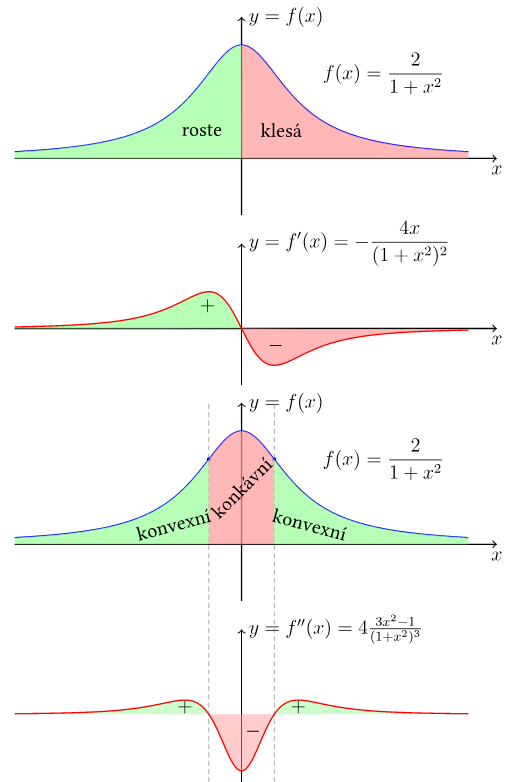
\includegraphics[width=.7\textwidth, center]{topics/bi-spol-34/images/prubeh.png}
\end{figure}

\newpage
\section{Tabulky}

\begin{figure}[h]
    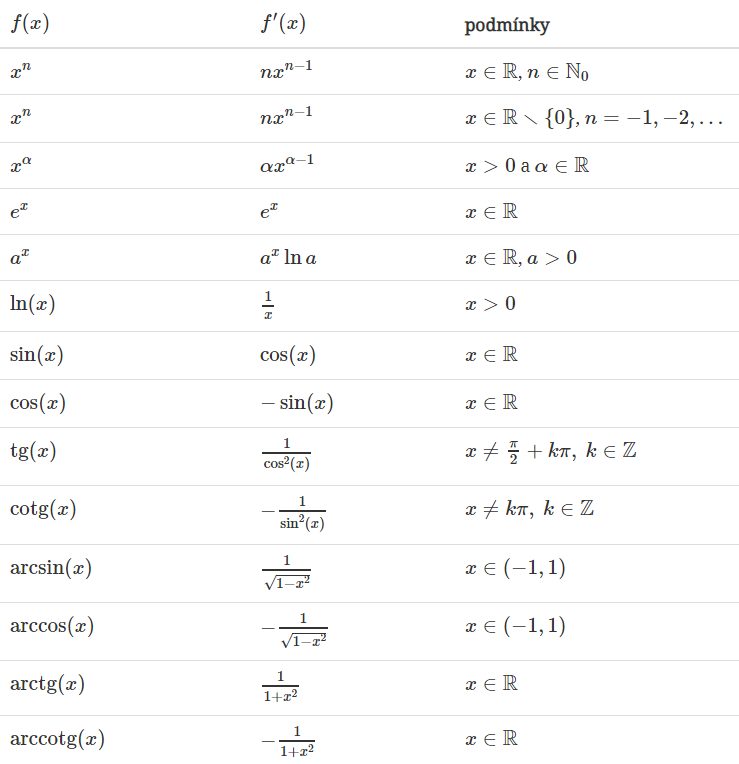
\includegraphics[width=\textwidth, center]{topics/bi-spol-34/images/derivace.png}
\end{figure}

\end{document}